%\section{Physics Object Reconstruction}
%\label{sec:obj}

The ATLAS detector serves to identify and measure the diverse fundamental particles—including photons, $e$, $\mu$, and $\tau$ leptons, alongside missing transverse energy and hadronic jets (which originate from quarks and gluons)—generated during high-energy $pp$ collisions, as depicted in the left panel of Figure~\ref{fig:coordinator}. To construct these sophisticated physics objects, the system must process and transform primitive detector readouts, encompassing collected charges, energy deposits, timing data, and hit patterns. This critical reconstruction procedure depends heavily on advanced algorithms, synergized with AI-driven methods, to guarantee highly accurate calorimetry and tracking. The essential sequential steps in this workflow involve executing a primary vertex reconstruction to isolate proton--proton interaction points, aggregating energy deposits within the calorimeters into dynamic clusters, generating tracks for charged particles throughout the Inner Detector and the Muon Spectrometer, and mathematically deriving the missing transverse energy ($E_{\text{T}}^{\text{miss}}$).

%This chapter presents the reconstruction of the primary physics objects used in the event selection. ATLAS coordinator for reconstruction is shown in the right panel of Figure~\ref{fig:coordinator}.
%The ATLAS experiment at the CERN Large Hadron Collider (LHC) employs a right-handed, cylindrical coordinate system to define the position of particles and detector components.

\begin{figure}[!htbp]
    \centering
    \subfloat[]{
    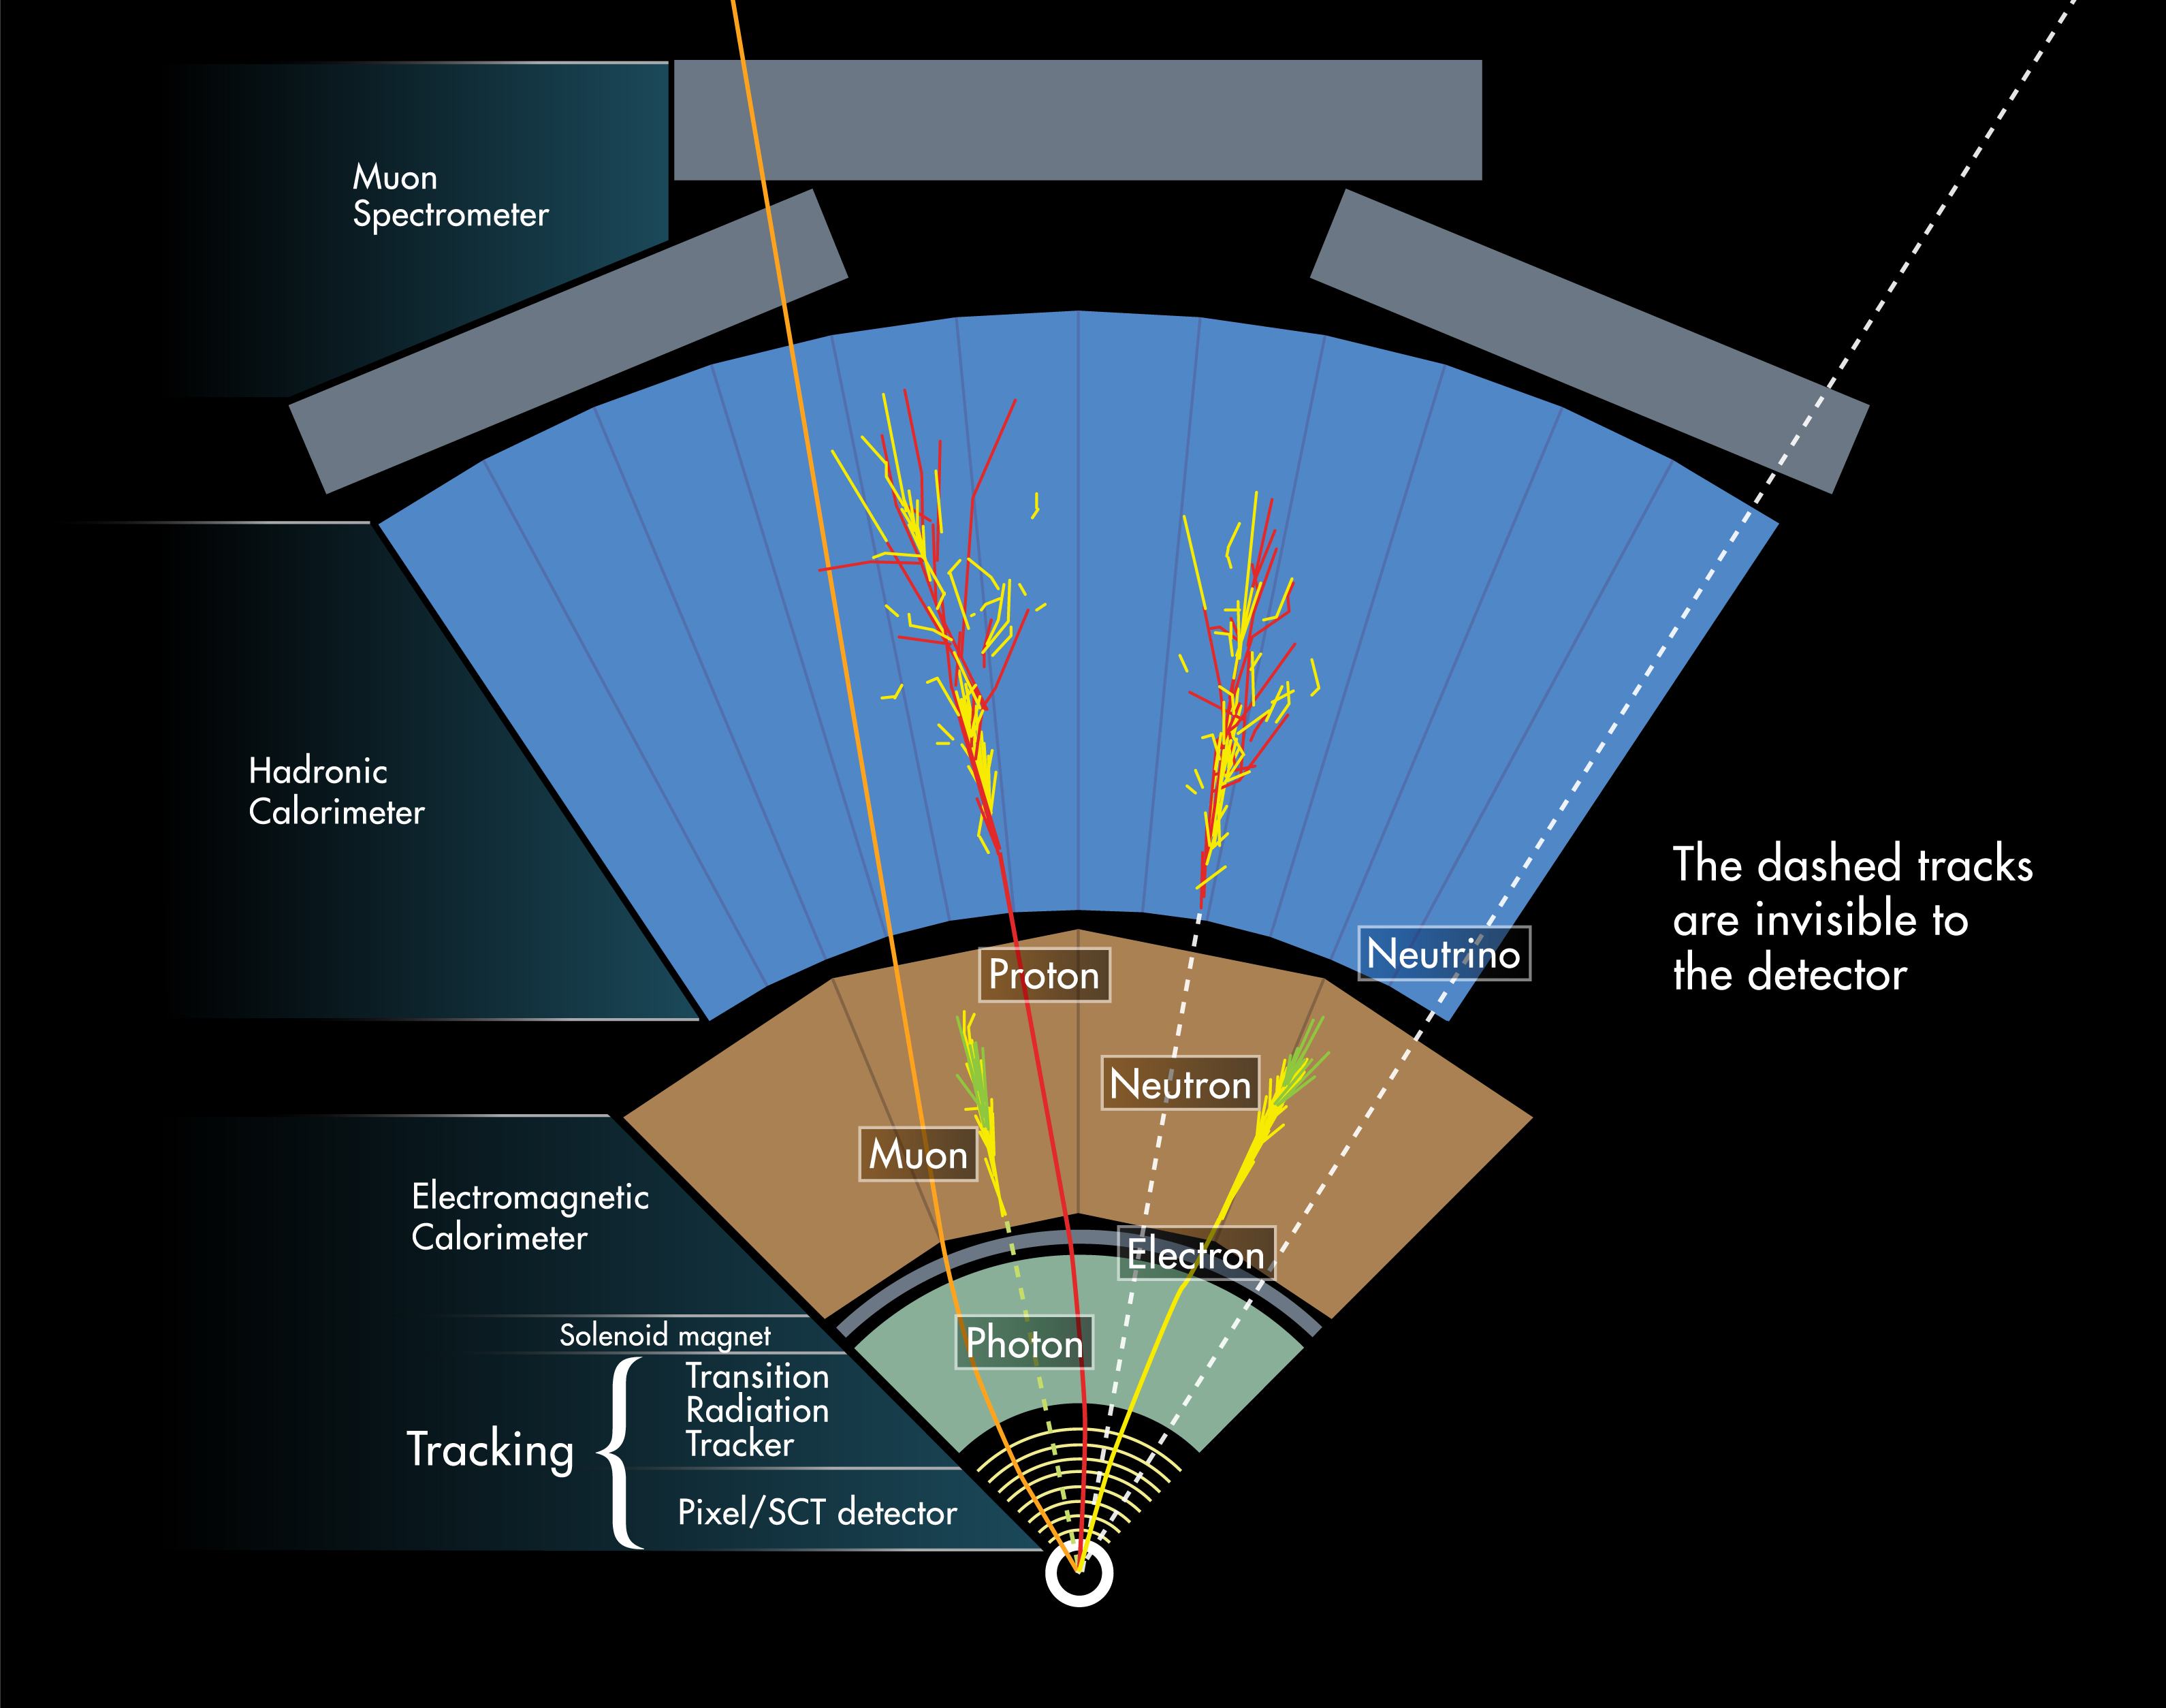
\includegraphics[width=0.43\textwidth]{figures/ch4-recon/particlepaths.jpg} 
    }
    \subfloat[]{
    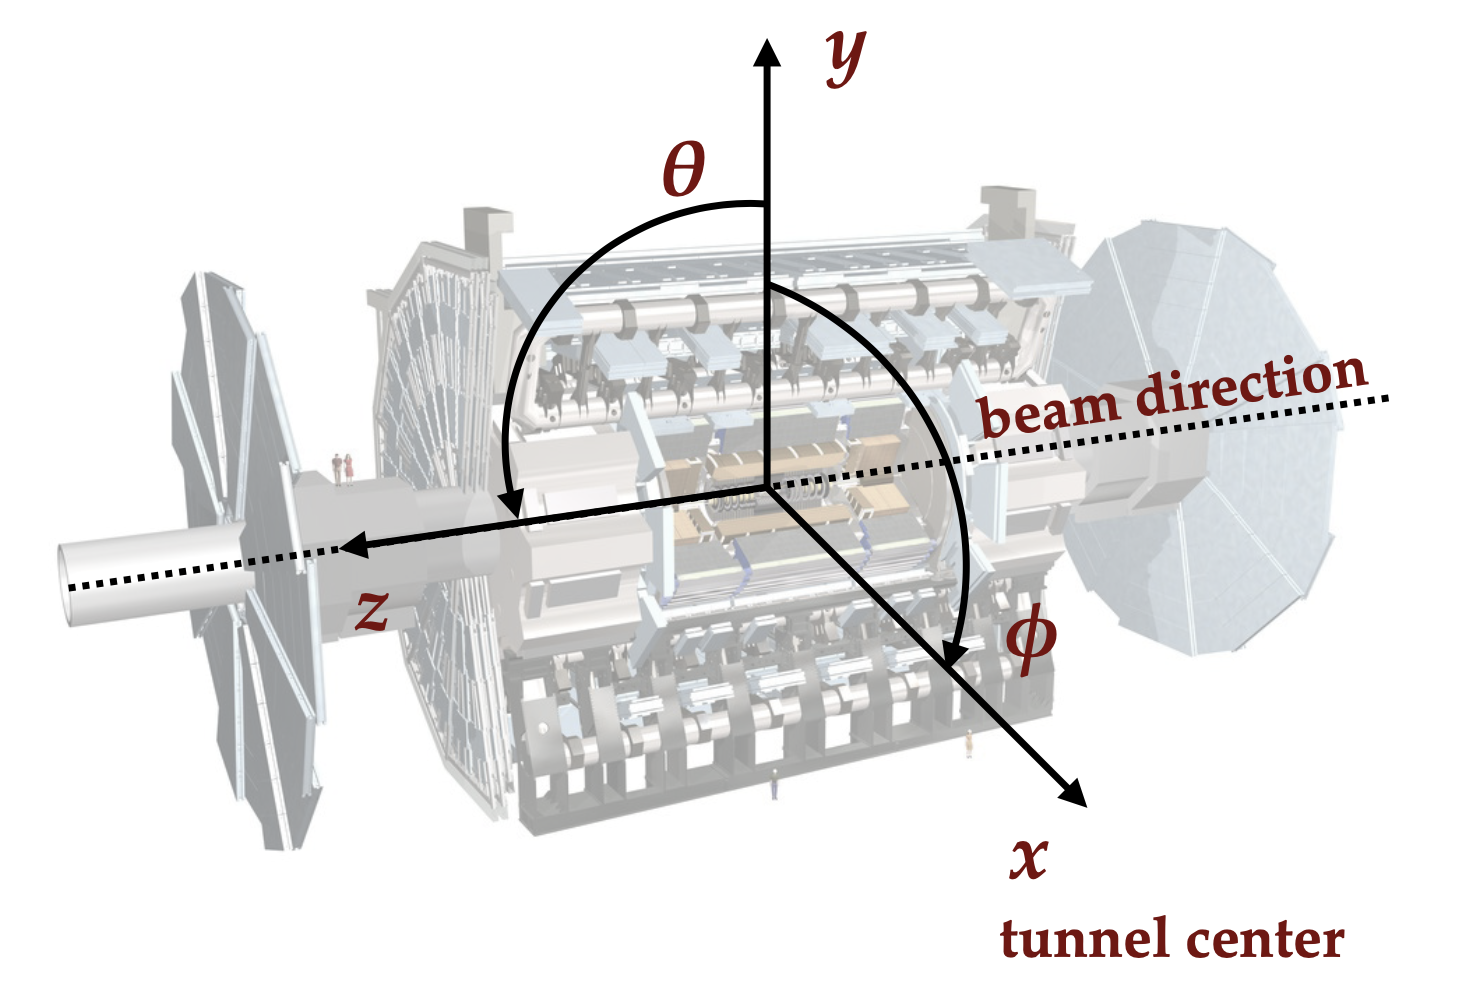
\includegraphics[width=0.55\textwidth]{figures/ch4-recon/ATLAS-coordinate.png}
    }
    \caption{(a) Illustration of the particles produced in the $pp$ collision passing the ATLAS sub-detector layers; (b) the ATLAS coordinate system for physics object reconstruction.}
    \label{fig:coordinator}
\end{figure}

%\subsection{Coordinate System}

As illustrated in Figure~\ref{fig:coordinator}(b), the ATLAS framework operates strictly on a right-handed Cartesian coordinate system. The absolute center of the detector acts as the origin point, representing the nominal interaction point (IP). The beam pipe establishes the orientation of the $z$-axis, with the positive and negative $z$ directions pointing directly toward side A and side C of the detector, respectively.
%
Meanwhile, the $x$-axis extends radially from the IP towards the geometric center of the LHC ring, whereas the $y$-axis is oriented vertically upwards towards the Earth's surface. The plane running orthogonal to the beam direction is recognized as the transverse ($x$--$y$) plane, where $r$ denotes the radial distance expanding outward from the beamline.

Spatial orientations are mapped utilizing the azimuthal angle $\phi$ alongside the polar angle $\theta$. To define positions in the transverse plane, the azimuthal angle $\phi$ is evaluated concentrically around the $z$-axis, usually restricted to the $[-\pi,\,\pi]$ interval. Conversely, the polar angle $\theta$ is derived by measuring the deflection from the positive $z$-axis.
%
Within the realm of experimental collider physics, researchers heavily favor the pseudorapidity metric $\eta$ over the standard polar angle $\theta$. This preference stems from the fact that spatial intervals measured in $\eta$ are mathematically invariant under longitudinal Lorentz boosts parallel to the beamline. The operational definition of pseudorapidity is given by the formula:
\begin{equation}
\eta = -\ln\left(\tan\frac{\theta}{2}\right).
\end{equation}

\section{Primary Vertex}

Identifying the precise three-dimensional spatial coordinates of the initial proton--proton collision is handled by the primary vertex reconstruction algorithm~\cite{ATLAS-PrimaryVertex-2017}, marking it as a critical baseline step in the ATLAS data pipeline. This method relies implicitly on the successful extraction of high-quality tracks built from inner tracking detector data. Initially, mathematical seeding algorithms group these particle tracks strictly according to their respective $z$-coordinates. Following this, an iterative fitting technique is applied to formulate potential candidate vertices. To properly mitigate the challenges posed by pile-up (the occurrence of simultaneous proton--proton interactions overlapping within a single bunch crossing), adaptive vertex-fitting logic is widely implemented.

For an event to be successfully flagged for selection, it must possess a minimum of one reconstructed collision vertex visibly linked to two or more tracks, with each track demonstrating a transverse momentum of $p_{\text{T}} > 0.5~\text{GeV}$. Out of all the viable candidate vertices, the one exhibiting the highest scalar sum of the squared transverse momenta derived from its associated tracks, $\sum p_{\text{T}}^2$, is officially designated as the primary vertex.

Any track formally linked to this primary vertex is strictly evaluated against stringent quality criteria concerning its impact parameters. Most notably, tight constraints are applied to the longitudinal impact parameter $z_0$. This variable quantifies the longitudinal distance (along the $z$-axis) separating the reconstructed primary vertex from the exact coordinate where the transverse impact parameter $d_0$ is evaluated. It must satisfy the condition:
\[
|z_0 \sin\theta| < 0.5~\text{mm},
\]
where $\theta$ represents the specific polar angle of the track relative to the beamline.

For all physics analyses presented within this thesis, it is absolutely mandatory that electron and muon candidates originate directly from the primary collision vertex. To enforce this, dedicated threshold cuts are imposed on the significance of the transverse impact parameter. Specifically, muon candidates must obey $|d_0/\sigma_{d_0}| < 3$, whereas electrons must satisfy $|d_0/\sigma_{d_0}| < 5$. In this context, $d_0$ represents the trajectory's transverse impact parameter evaluated against the established beamline axis, with $\sigma_{d_0}$ acting as its measured statistical uncertainty.

\section{Electrons}
The standard protocol for extracting electrons in the ATLAS experiment~\cite{ATLAS-Egamma-2019} hinges on the spatial pairing of trajectories from the Inner Detector (ID) with isolated energy clusters formed within the electromagnetic (EM) calorimeter. To dynamically aggregate the scattered energy deposits generated by EM showers, a specialized supercluster algorithm is deployed. This strategy yields an excellent reconstruction efficiency for electrons possessing a transverse energy $E_{\text{T}}$ greater than a few GeV.

\begin{figure}[!htbp]
    \centering
    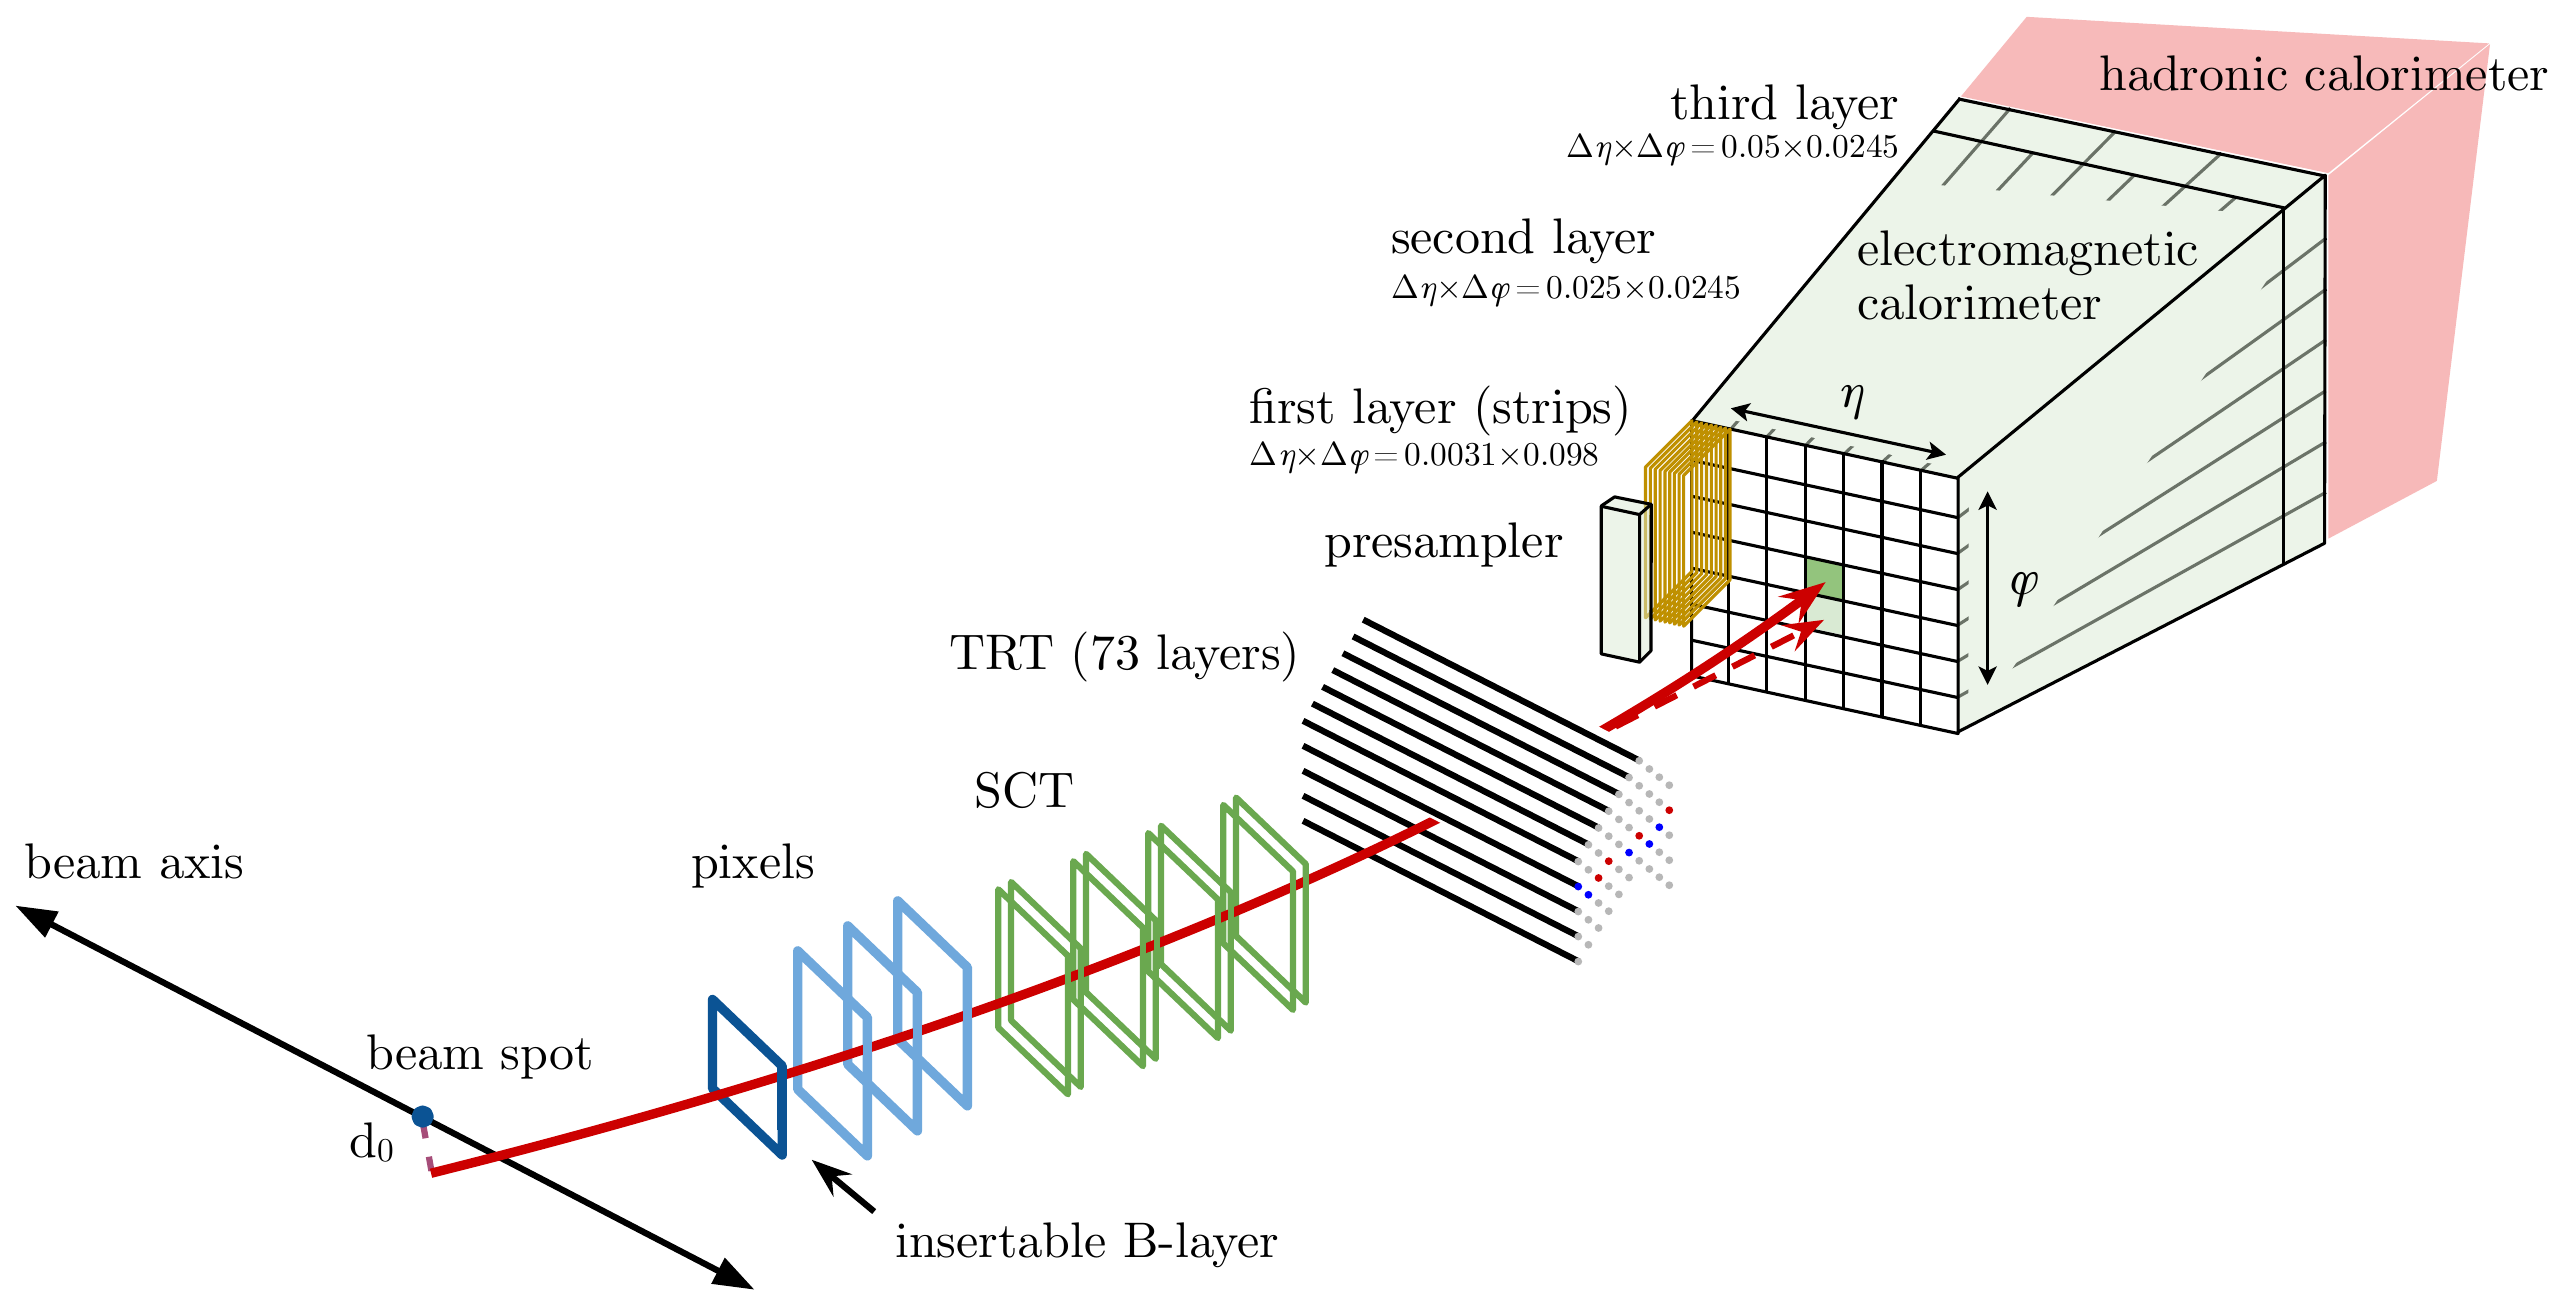
\includegraphics[width=0.8\textwidth]{figures/ch4-recon/Obj-electron-flow.png}
    \caption{Diagrammatic representation of the detector sub-systems involved in reconstructing electrons, illustrating the alignment of electromagnetic (EM) calorimeter energy clusters with Inner Detector (ID) trajectories.}
    \label{fig:e-ID}
\end{figure}

As conveyed in Figure~\ref{fig:e-ID}, valid electron candidates are assembled whenever an EM calorimeter cluster can be geometrically synchronized with an ID track. The subsequent electron identification phase utilizes a sophisticated likelihood-based discriminant, which mathematically synthesizes several variables: the spatial quality of the track-cluster alignment, intrinsic track characteristics, and the topological profile of the EM shower. A discrete set of standardized identification working points is established by the collaboration, namely \texttt{Loose}, \texttt{Medium}, and \texttt{Tight}~\cite{ATLAS-Egamma-2019}. 
\begin{figure}[!htbp]
    \centering
    \subfloat[] {
    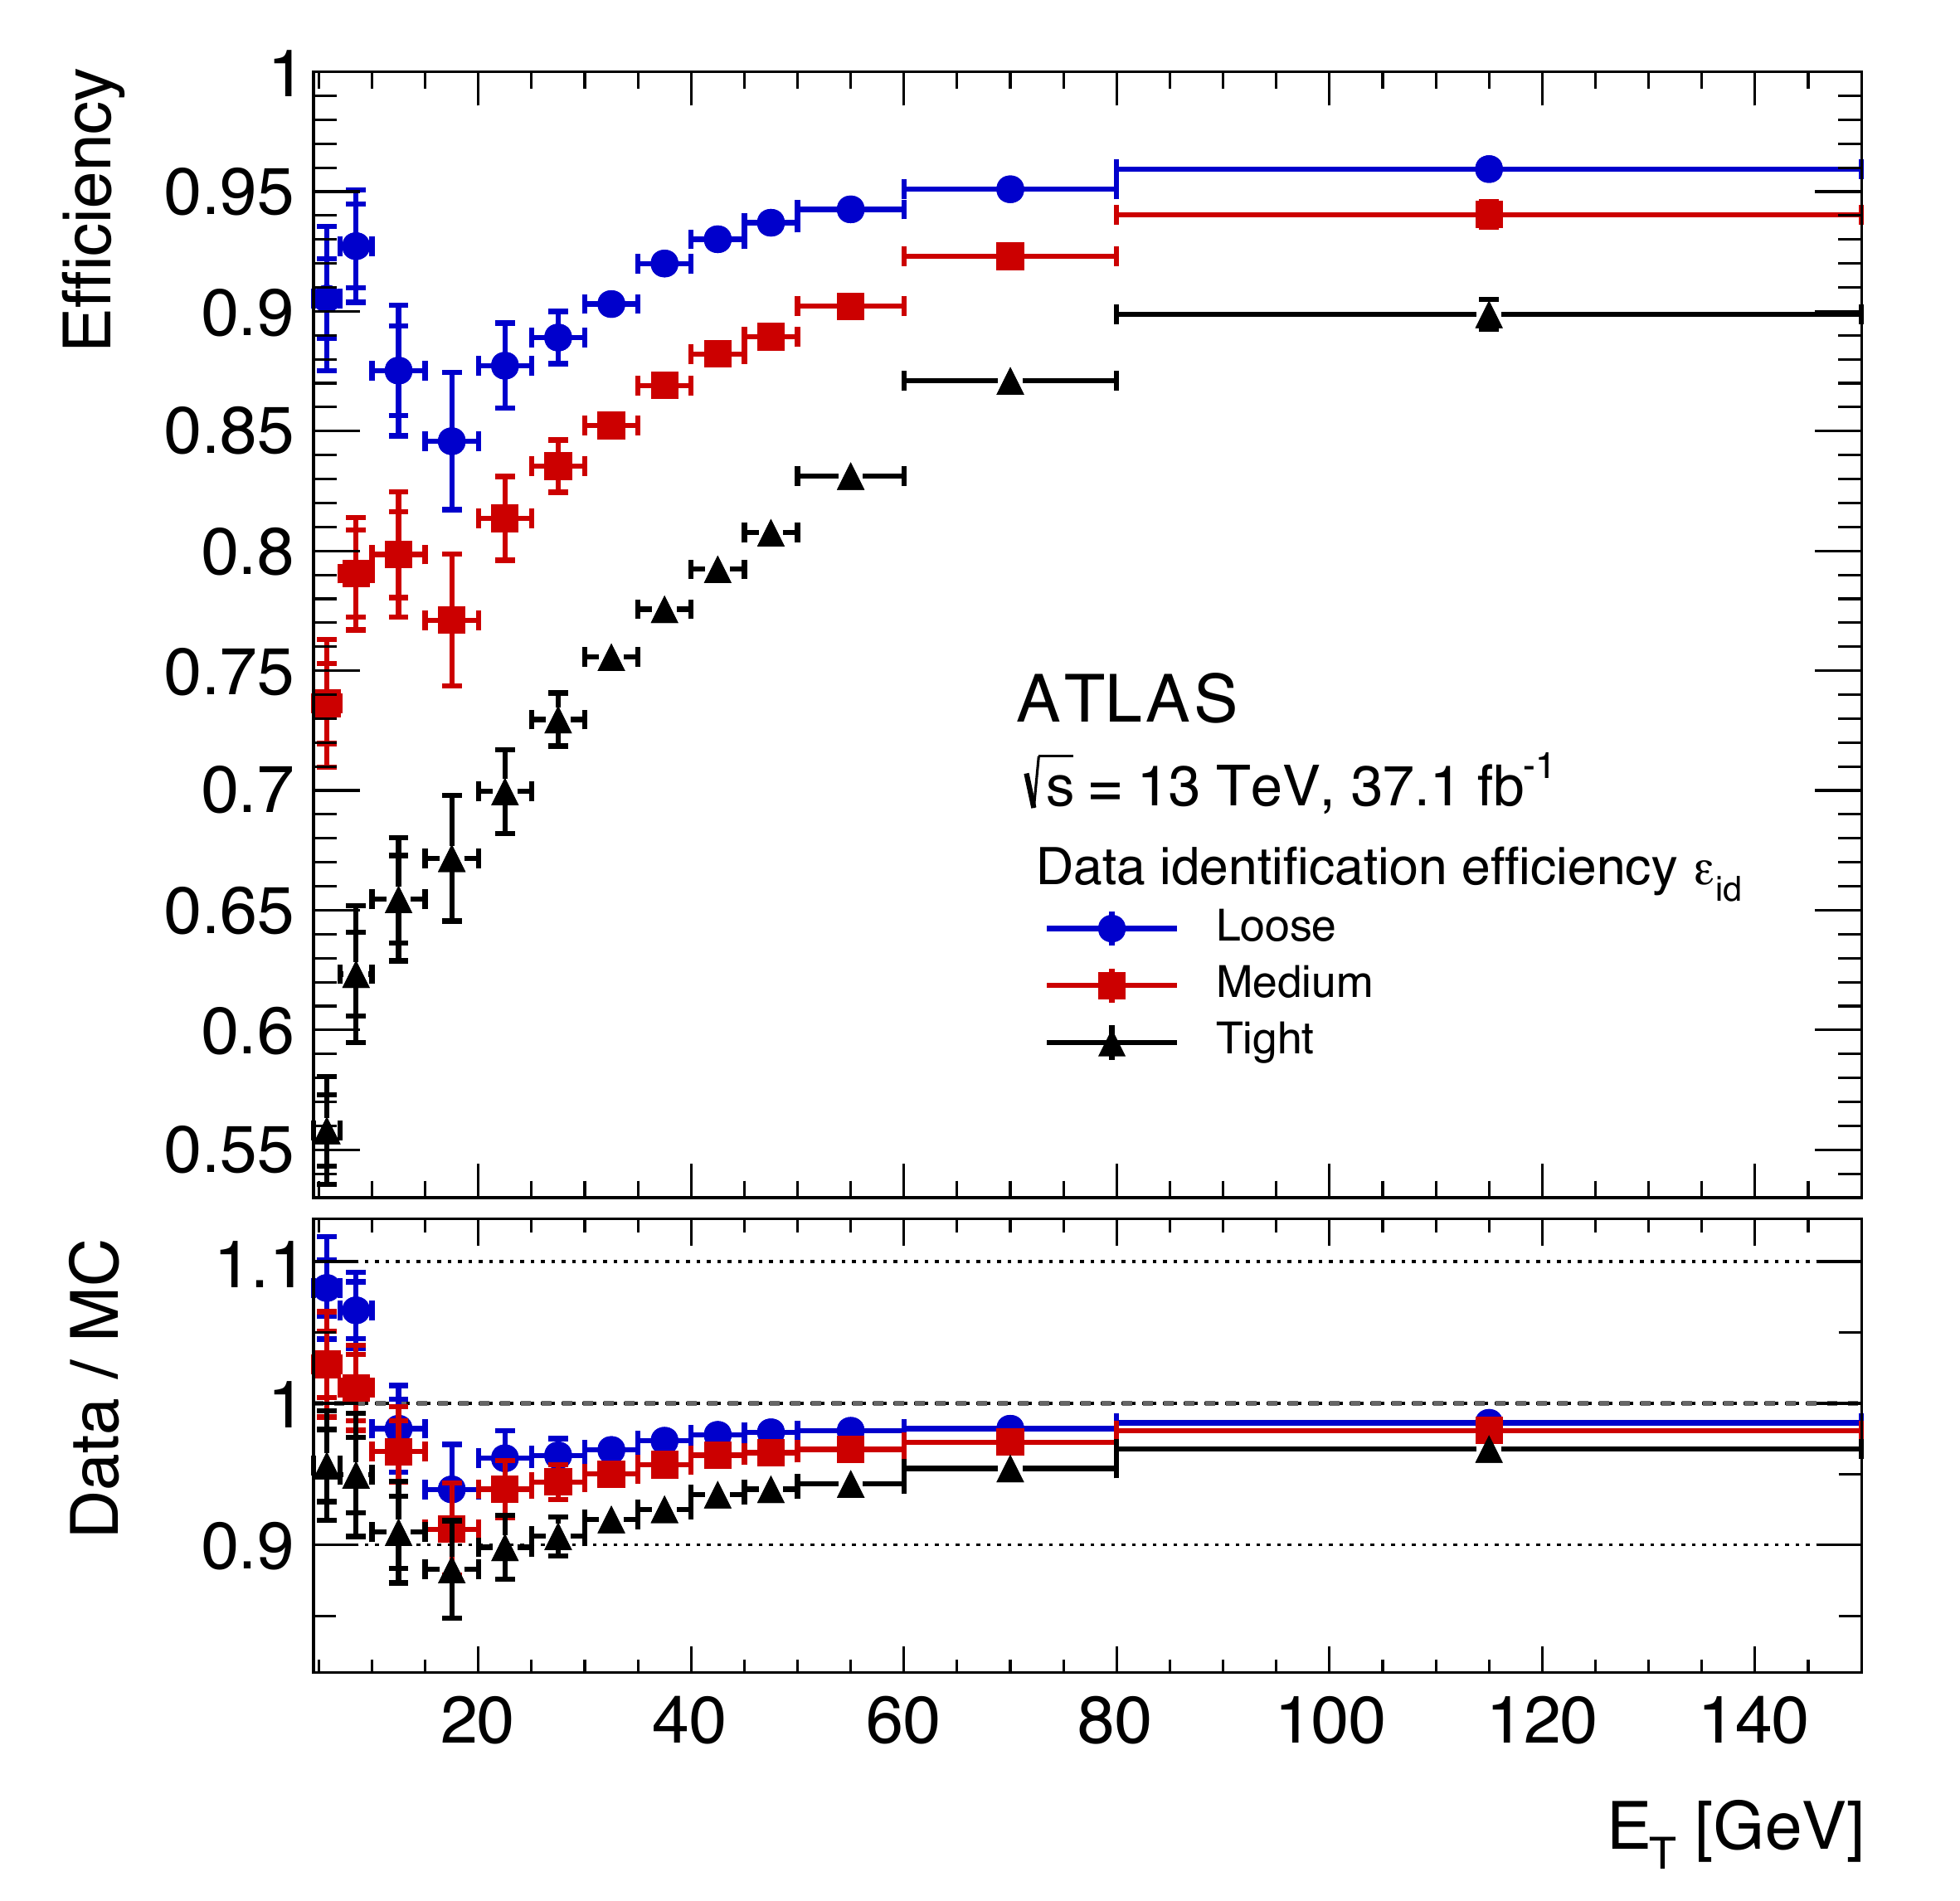
\includegraphics[width=0.45\textwidth]{figures/ch4-recon/Obj-eID-eff-ET.png}
    }
    \subfloat[] {
    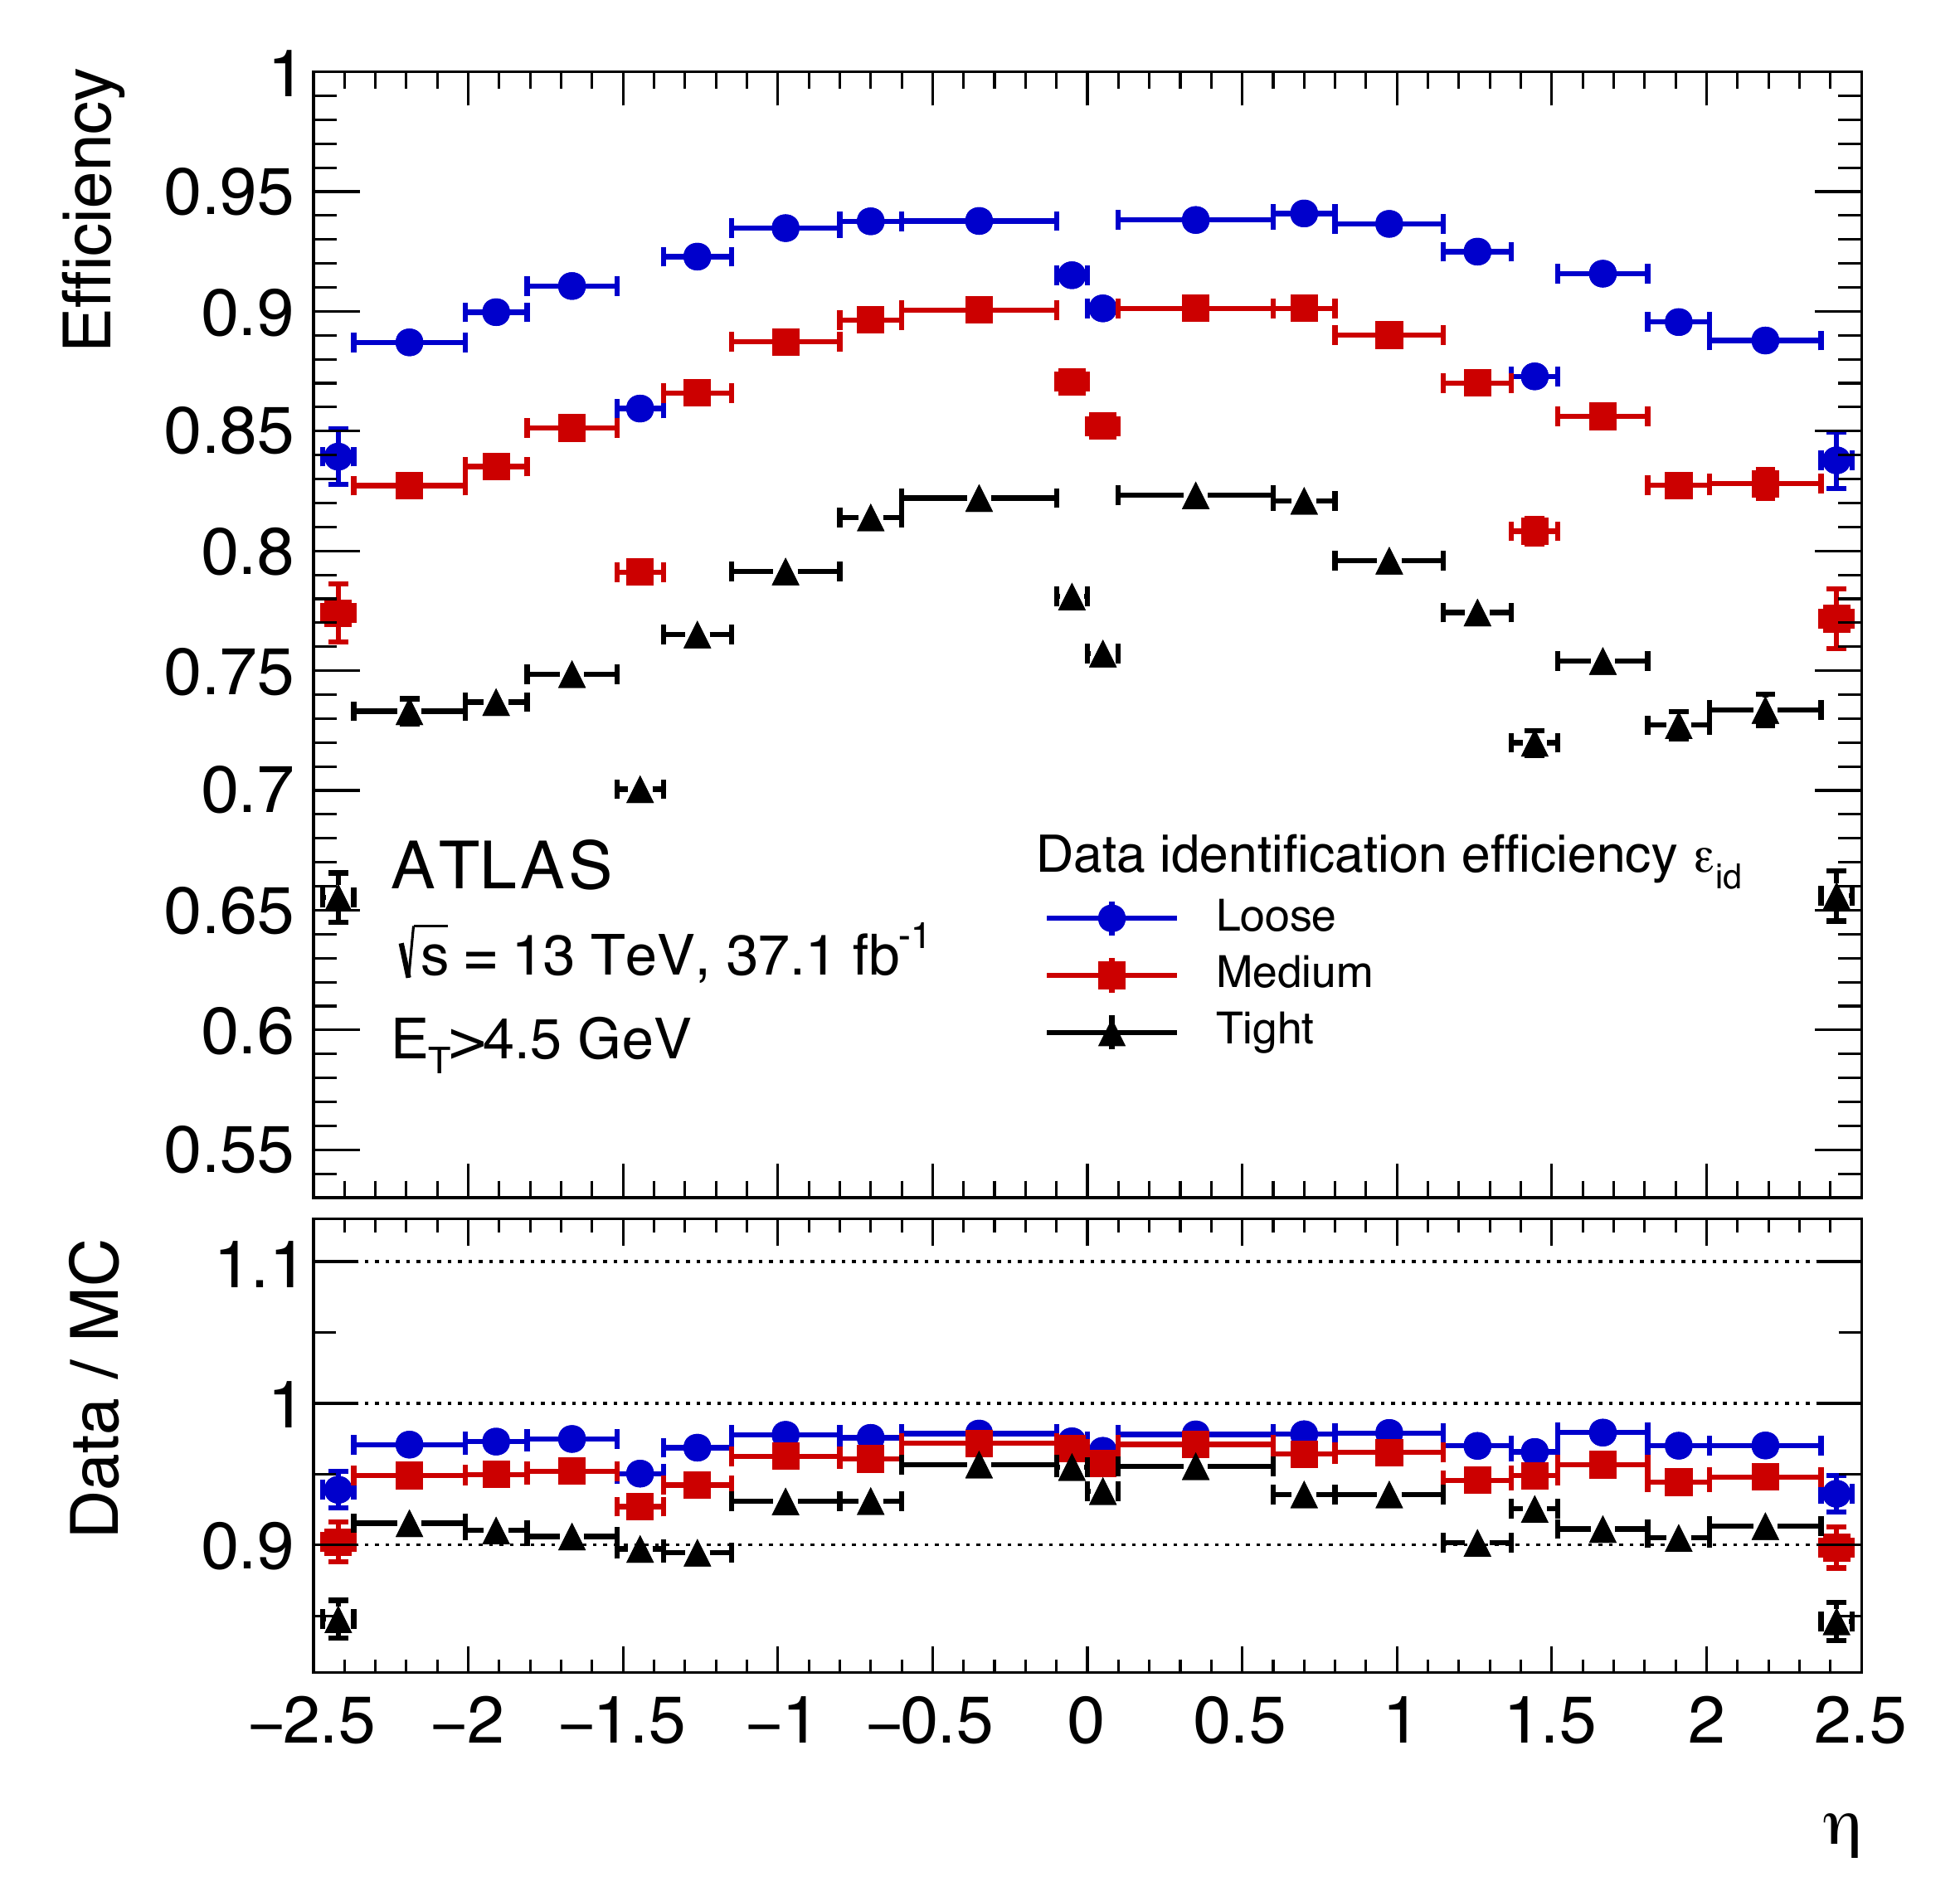
\includegraphics[width=0.45\textwidth]{figures/ch4-recon/Obj-eID-eff-eta.png}
    }
    \caption{Performance profiles showing the efficiency of electron reconstruction and identification, evaluated against the electron's transverse energy $E_{\text{T}}$ (a) and its pseudorapidity $\eta$ (b).}
    \label{fig:eID-eff}
\end{figure}
The data-driven studies outlined in this document mandate that all accepted electrons satisfy the \texttt{Medium} likelihood-based identification threshold. By adopting this specific operational working point, the analyses benefit from an average identification efficiency hovering around $90\%$~\cite{ATLAS-Egamma-Efficiencies-2024}, a performance trend visibly charted in Figure~\ref{fig:eID-eff}. To accurately evaluate the electron's final momentum, the energy magnitude recorded by the calorimeter cluster is fused with the directional trajectory provided by the matched track.

Additionally, eligible electron candidates must be captured within the highly sensitive fiducial volume of the detector, requiring their measured cluster pseudorapidity to remain within $|\eta| < 2.47$. As a strict caveat, any candidates falling into the geometric transition gap separating the barrel and endcap calorimeters ($1.37 < |\eta| < 1.52$) are explicitly vetoed.

Furthermore, to stringently mitigate background contamination arising from non-prompt leptons and stray hadronic jets, an isolation requirement is enforced. Electrons must remain adequately separated from one another and from surrounding activity, cleanly fulfilling the designated particle-flow isolation standards~\cite{ATLAS-Egamma-Efficiencies-2024}. This determination is calculated by cross-referencing inner detector track data alongside clustered energy deposits found in the calorimeters. 

\section{Muons}

When it comes to muon reconstruction, the dedicated ATLAS framework~\cite{ATLAS-Muon-Reco-ID-2021} deploys a multi-layered analytical strategy. By robustly integrating telemetry from both the Muon Spectrometer (MS) and the Inner Detector (ID), the system routinely achieves an identification efficiency peaking near $98\%$ (consult Figure~\ref{fig:mu-ID} for the layout). Muon tracks are fundamentally categorized into four primary reconstruction archetypes: Combined (CB), Standalone (SA), Segment-Tagged (ST), and Calorimeter-Tagged (CT). Among these, Combined muons offer the most optimal signal-to-background separation, especially for candidates registering a muon $p_{\text{T}} > 20~\text{GeV}$.
This reconstruction sequence initiates by locating track segments within the MS, projecting their flight paths back to the beamline (while actively adjusting for expected material energy losses), and ultimately pairing them directly with corresponding ID tracks.
\begin{figure}[!htbp]
    \centering
    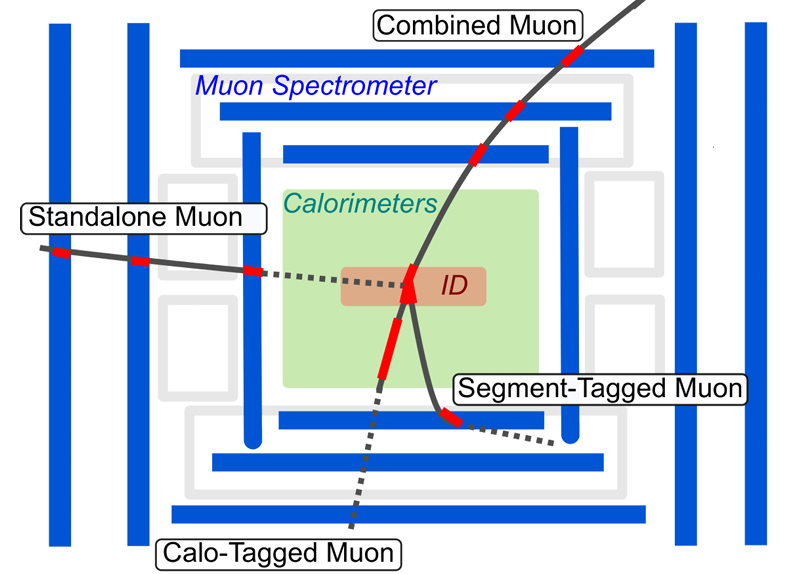
\includegraphics[width=0.6\textwidth]{figures/ch4-recon/Muon-recon.png}
    \caption{Visual breakdown of the detector components utilized for isolating muons. The classification of a muon candidate depends directly on which tracking sub-systems contribute to its reconstruction. \textit{Combined} muons successfully merge trajectory data from both the Muon Spectrometer and the Inner Detector. \textit{Standalone} muons are built exclusively from Muon Spectrometer hits. \textit{Segment-Tagged} candidates pair an Inner Detector track with just one localized track segment in the Muon Spectrometer. Finally, \textit{Calorimeter-Tagged} muons rely on an Inner Detector trajectory combined with a distinct minimum-ionizing energy signature deposited within the calorimeter volume.}
    \label{fig:mu-ID}
\end{figure}

To accurately calibrate the overall scale and resolution of the measured muon momentum, physicists exploit well-understood $\text{Z} \to \mu^+\mu^-$ and $\text{J}/\psi \to \mu^+\mu^-$ decay topologies. Figure~\ref{fig:mu-ID2} displays how the underlying reconstruction efficiency scales according to the muon's pseudorapidity $\eta$ and transverse momentum $p_{\text{T}}$.

Across the various experimental studies documented in this thesis, muon candidates are strictly filtered using the \texttt{Medium} identification benchmark~\cite{ATLAS-Muon-Reco-ID-2021}. This standard enforces rigid minimum hit-count thresholds simultaneously in the MS and the ID~\cite{ATLAS-CONF-2020-030}. The final momentum assignment for a given muon merges the MS measurements—corrected for any minor energy amounts deposited in the calorimeters—with the core ID track parameters. Additionally, valid muon pseudorapidity is restricted to the $|\eta| < 2.5$ window.

\begin{figure}[!htbp]
    \centering
        \subfloat[] {
    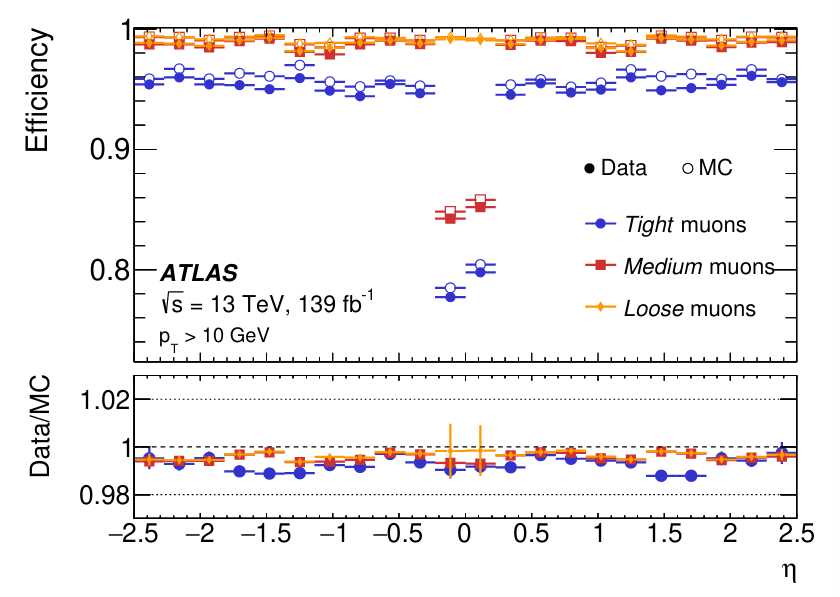
\includegraphics[width=0.48\textwidth]{figures/ch4-recon/Muon-eff-eta.png}
    }
        \subfloat[] {
    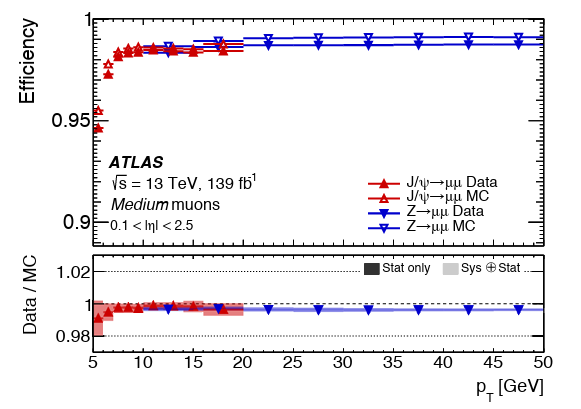
\includegraphics[width=0.48\textwidth]{figures/ch4-recon/Muon-eff-pT.png}
    }
    \caption{Muon reconstruction and identification performance scaling mapped as a function of $\eta$ (a) and $p_{\text{T}}$ (b).}
    \label{fig:mu-ID2}
\end{figure}

%%%%%%%%%%%%%%%
Prompt muons originating directly from the decay of $\text{W}$ and $\text{Z}$ bosons tend to be highly isolated. 
Consequently, this thesis mandates that muon candidates maintain strict isolation from each other and surrounding particles. This status is verified by ensuring they pass the designated particle-flow isolation criteria~\cite{ATLAS-Muon-Isolation-PFlow-2021}, which evaluate surrounding inner detector track densities alongside calorimeter energy clusters. 

\section{Jets}
Following their generation during inelastic hadron collisions, free gluons and quarks instantaneously undergo hadronization, which manifests physically as complex hadronic jets. The algorithmic process of reconstructing these composite jets merges localized topological energy clusters collected by the electromagnetic and hadronic calorimeters with precise trajectory data supplied by the Inner Detector.

To assemble these jets, the ATLAS collaboration overwhelmingly employs the anti-$k_t$ clustering algorithm~\cite{Cacciari:2008gp}. The defining parameter governing this algorithm is the angular distance multiplier $R$, which effectively dictates the radial size of the jet and acts as the strict spatial threshold for absorbing neighboring particles and energy clusters. Jets characterized by a narrow cone, or small-$R$ jets, are typically seeded by individual gluons or quarks and are clustered via the anti-$k_t$ algorithm restricted to a radius of $R=0.4$. Conversely, large-$R$ jets ($R=1.0$) are deployed primarily to capture the merged hadronic decay products resulting from massive boosted particles, such as Higgs bosons, top quarks, and $\text{W}$/$\text{Z}$ bosons.

For jets that satisfy the kinematic bounds of $p_{\text{T}} > 30~\text{GeV}$ alongside $|\eta| < 4.5$, the anti-$k_t$ algorithm is fed using particle-flow (PFlow) objects~\cite{ATLAS-PFlow-Jets-2017}. These PFlow objects intelligently cross-reference ID tracks with calorimeter deposits to drastically refine the evaluation of jet kinematics. The baseline jet energy scale (JES) calibration is extracted initially from Monte Carlo simulations. Subsequently, this scale is dynamically fine-tuned using data-driven in situ calibration techniques, heavily exploiting the well-measured kinematics of $\text{Z}+$jet, $\gamma+$jet, and dijet events~\cite{JETM-2018-05}.

To heavily mitigate the impact of pile-up interactions, a jet-vertex tagger (JVT)~\cite{ATLAS-CONF-2014-018} requirement is strictly imposed on any jet falling into the $p_{\text{T}} < 60~\text{GeV}$ and $|\eta| < 2.4$ regime.

Whenever an analysis deeply depends on tracking hadronic final states, the systematic uncertainties tied to both the jet energy resolution (JER) and the jet energy scale (JES) frequently emerge as the most dominant sources of experimental error. The fractional resolution of the ATLAS small-$R$ jet energy, plotted against the transverse momentum $p_{\text{T}}$, is illustrated in Figure~\ref{fig:JER}~\cite{ATLAS-Jet-JER-2021}.
\begin{figure}[!htbp]
    \centering
    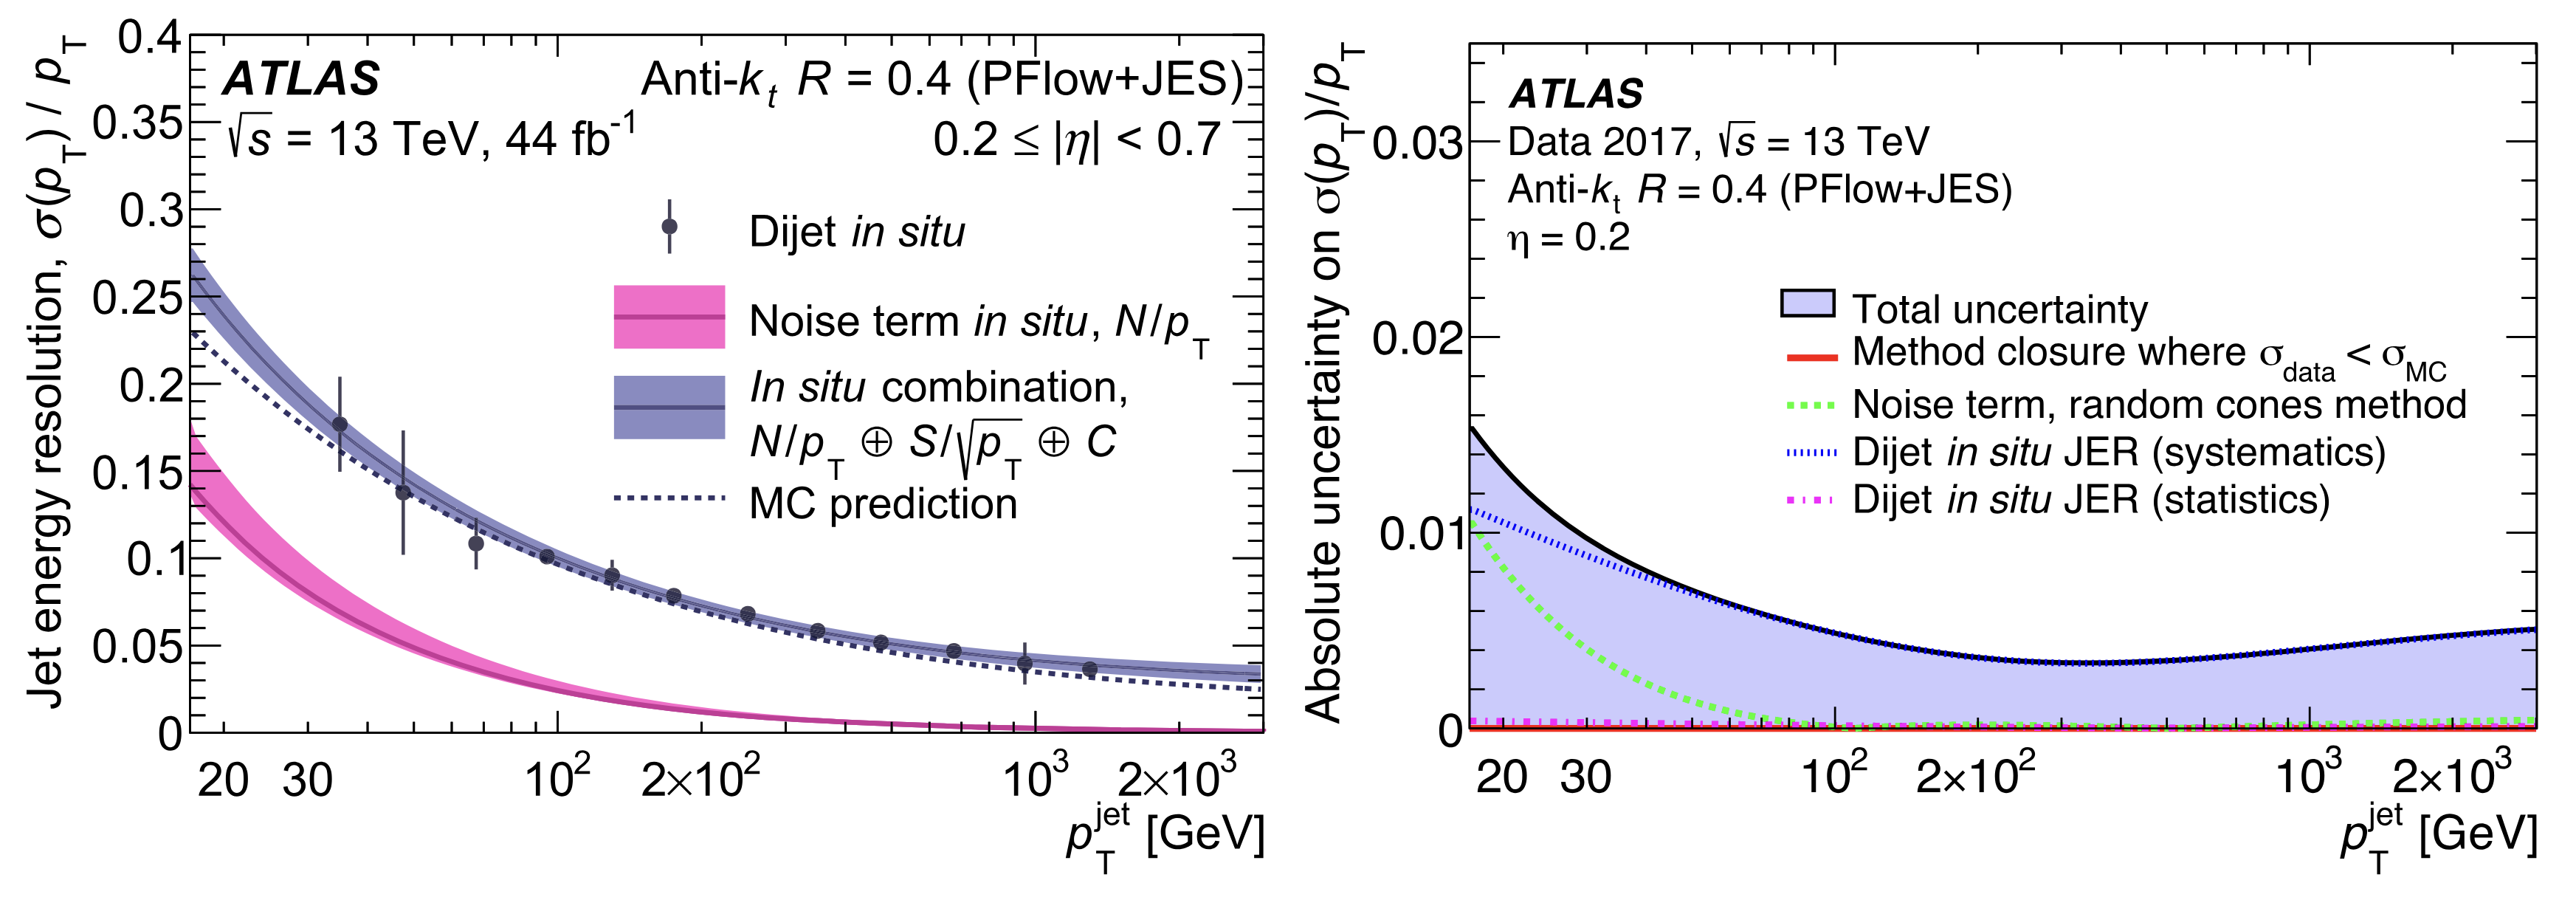
\includegraphics[width=0.90\textwidth]{figures/ch4-recon/JERpTanduncertainty.png}
    \caption{The fractional energy resolution for standard jets, plotted against the transverse momentum $p_{\text{T}}$. These performance curves are shown for (a) the pseudorapidity interval $0.2 < |\eta| < 0.7$ and (b) a specific target of $\eta = 0.2$.}
    \label{fig:JER}
\end{figure}

Additionally, to successfully tag jets that harbor $b$-hadrons, researchers deploy the \texttt{DL1r} multivariate $b$-tagging framework~\cite{FTAG-2020-08, FTAG-2019-02}. This tool is applied exclusively to jets that surpass the kinematic thresholds of $p_{\text{T}} > 20~\text{GeV}$ and fall within $|\eta| < 2.5$. The analyses presented in this thesis adopt the 85\% efficiency working point. Operating at this specific threshold, the algorithm reliably yields a rejection factor of 6.3 for $c$-jets and up to 33 for standard light-flavour jets.

%Overlaps between reconstructed objects are accounted for with a removal procedure that is mainly based on the angular separation between the different final-state objects (electrons, muons, jets). The procedure is the same as the one described in Ref.~\cite{ATLAS2016-overlap}.

\section{Missing Transverse Energy}
Due to their weakly interacting nature, final-state neutrinos ($\nu$) easily penetrate the entire ATLAS detector volume without triggering any hardware sensors, making direct reconstruction impossible.
\begin{figure}[!htbp]
    \centering
    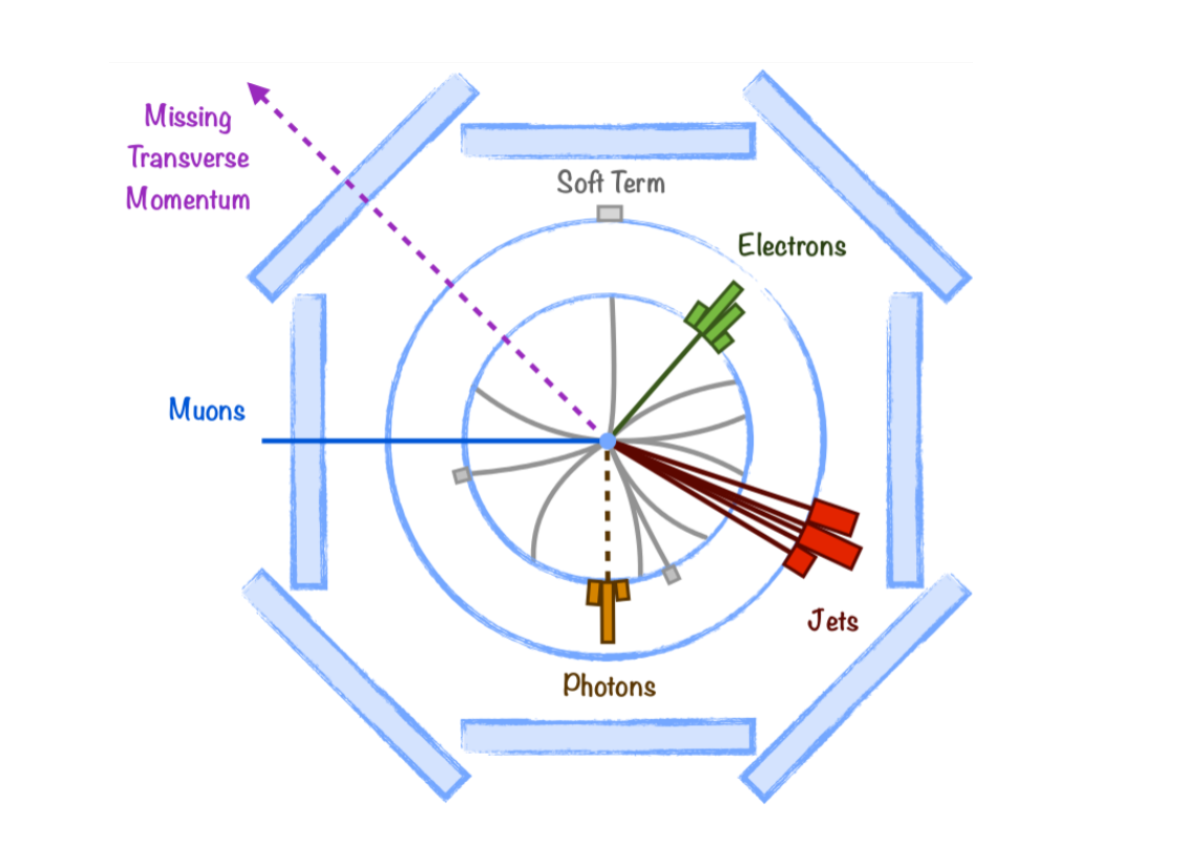
\includegraphics[width=0.75\textwidth]{figures/ch4-recon/Obj-met-diagram.png}   
    \caption{Vectorial derivation of the missing transverse energy, illustrating how it balances against the combined transverse momenta of all successfully reconstructed jets and leptons.}
    \label{fig:met}
\end{figure}
 Instead, their unseen presence is mathematically deduced via the $E_{\text{T}}^{\text{miss}}$ parameter. This variable is derived by calculating the magnitude of the negative vectorial sum of the transverse momenta generated by all fully identified physics objects (namely, leptons and jets). To ensure absolute momentum conservation, this calculation also integrates any residual unassociated tracks that clearly map back to the primary collision vertex~\cite{JETM-2020-03}, as mathematically structured in Equation~\eqref{eq:Et-miss}. 

\begin{equation} \label{eq:Et-miss}
    \vec{E}_{\text{T}}^{\text{miss}} = - \sum_{\text{electrons}} \vec{p}_{\text{T}}^{\,e} - \sum_{\text{photons}} \vec{p}_{\text{T}}^{\,\gamma} - \sum_{\tau\text{-leptons}} \vec{p}_{\text{T}}^{\,\tau_{\text{had}}} - \sum_{\text{muons}} \vec{p}_{\text{T}}^{\,\mu} - \sum_{\text{jets}} \vec{p}_{\text{T}}^{\,\text{jet}} - \sum_{\text{unused tracks}} \vec{p}_{\text{T}}^{\,\text{track}}.
\end{equation} 

As visually demonstrated in Figure~\ref{fig:met}, the missing transverse energy, $E_{\text{T}}^{\text{miss}}$, is physically oriented in the direction directly opposite to the combined vector sum of all other visible particles in the event.

Working in tandem with $E_{\text{T}}^{\text{miss}}$, modern event selection topologies frequently incorporate the total transverse energy metric, $H_{\text{T}}$. This value is obtained straightforwardly by computing the scalar sum of the transverse momenta contributed by every explicitly verified jet and lepton currently selected for the analysis.